\section{Robot} 

The robot is made using a Lego Mindstorm kit, with a NXT brick and a few different sensors, like light sensors, push sensors, etc. There was also a lot of Lego at disposal so there were free reins, construction wise. Sensor wise there were more limitations, i.e. only sensors from the given kit could be used.
\subsection{Behavior}

\subsection{Construction}
The skeleton of the robot was designed to be as low as possible, in order to get the light sensors as close to the ground as possible. A side effect of this is that it makes the robot more stable when turning. In front of the robot a gripper was placed, with room for two sensors in between the robot and the gripper. The final choice of design and sensor placement can be seen in figure \ref{fig:final_robot}. Other constructions was tried, but discarded for different reasons.

\begin{figure}[H]
\centering
 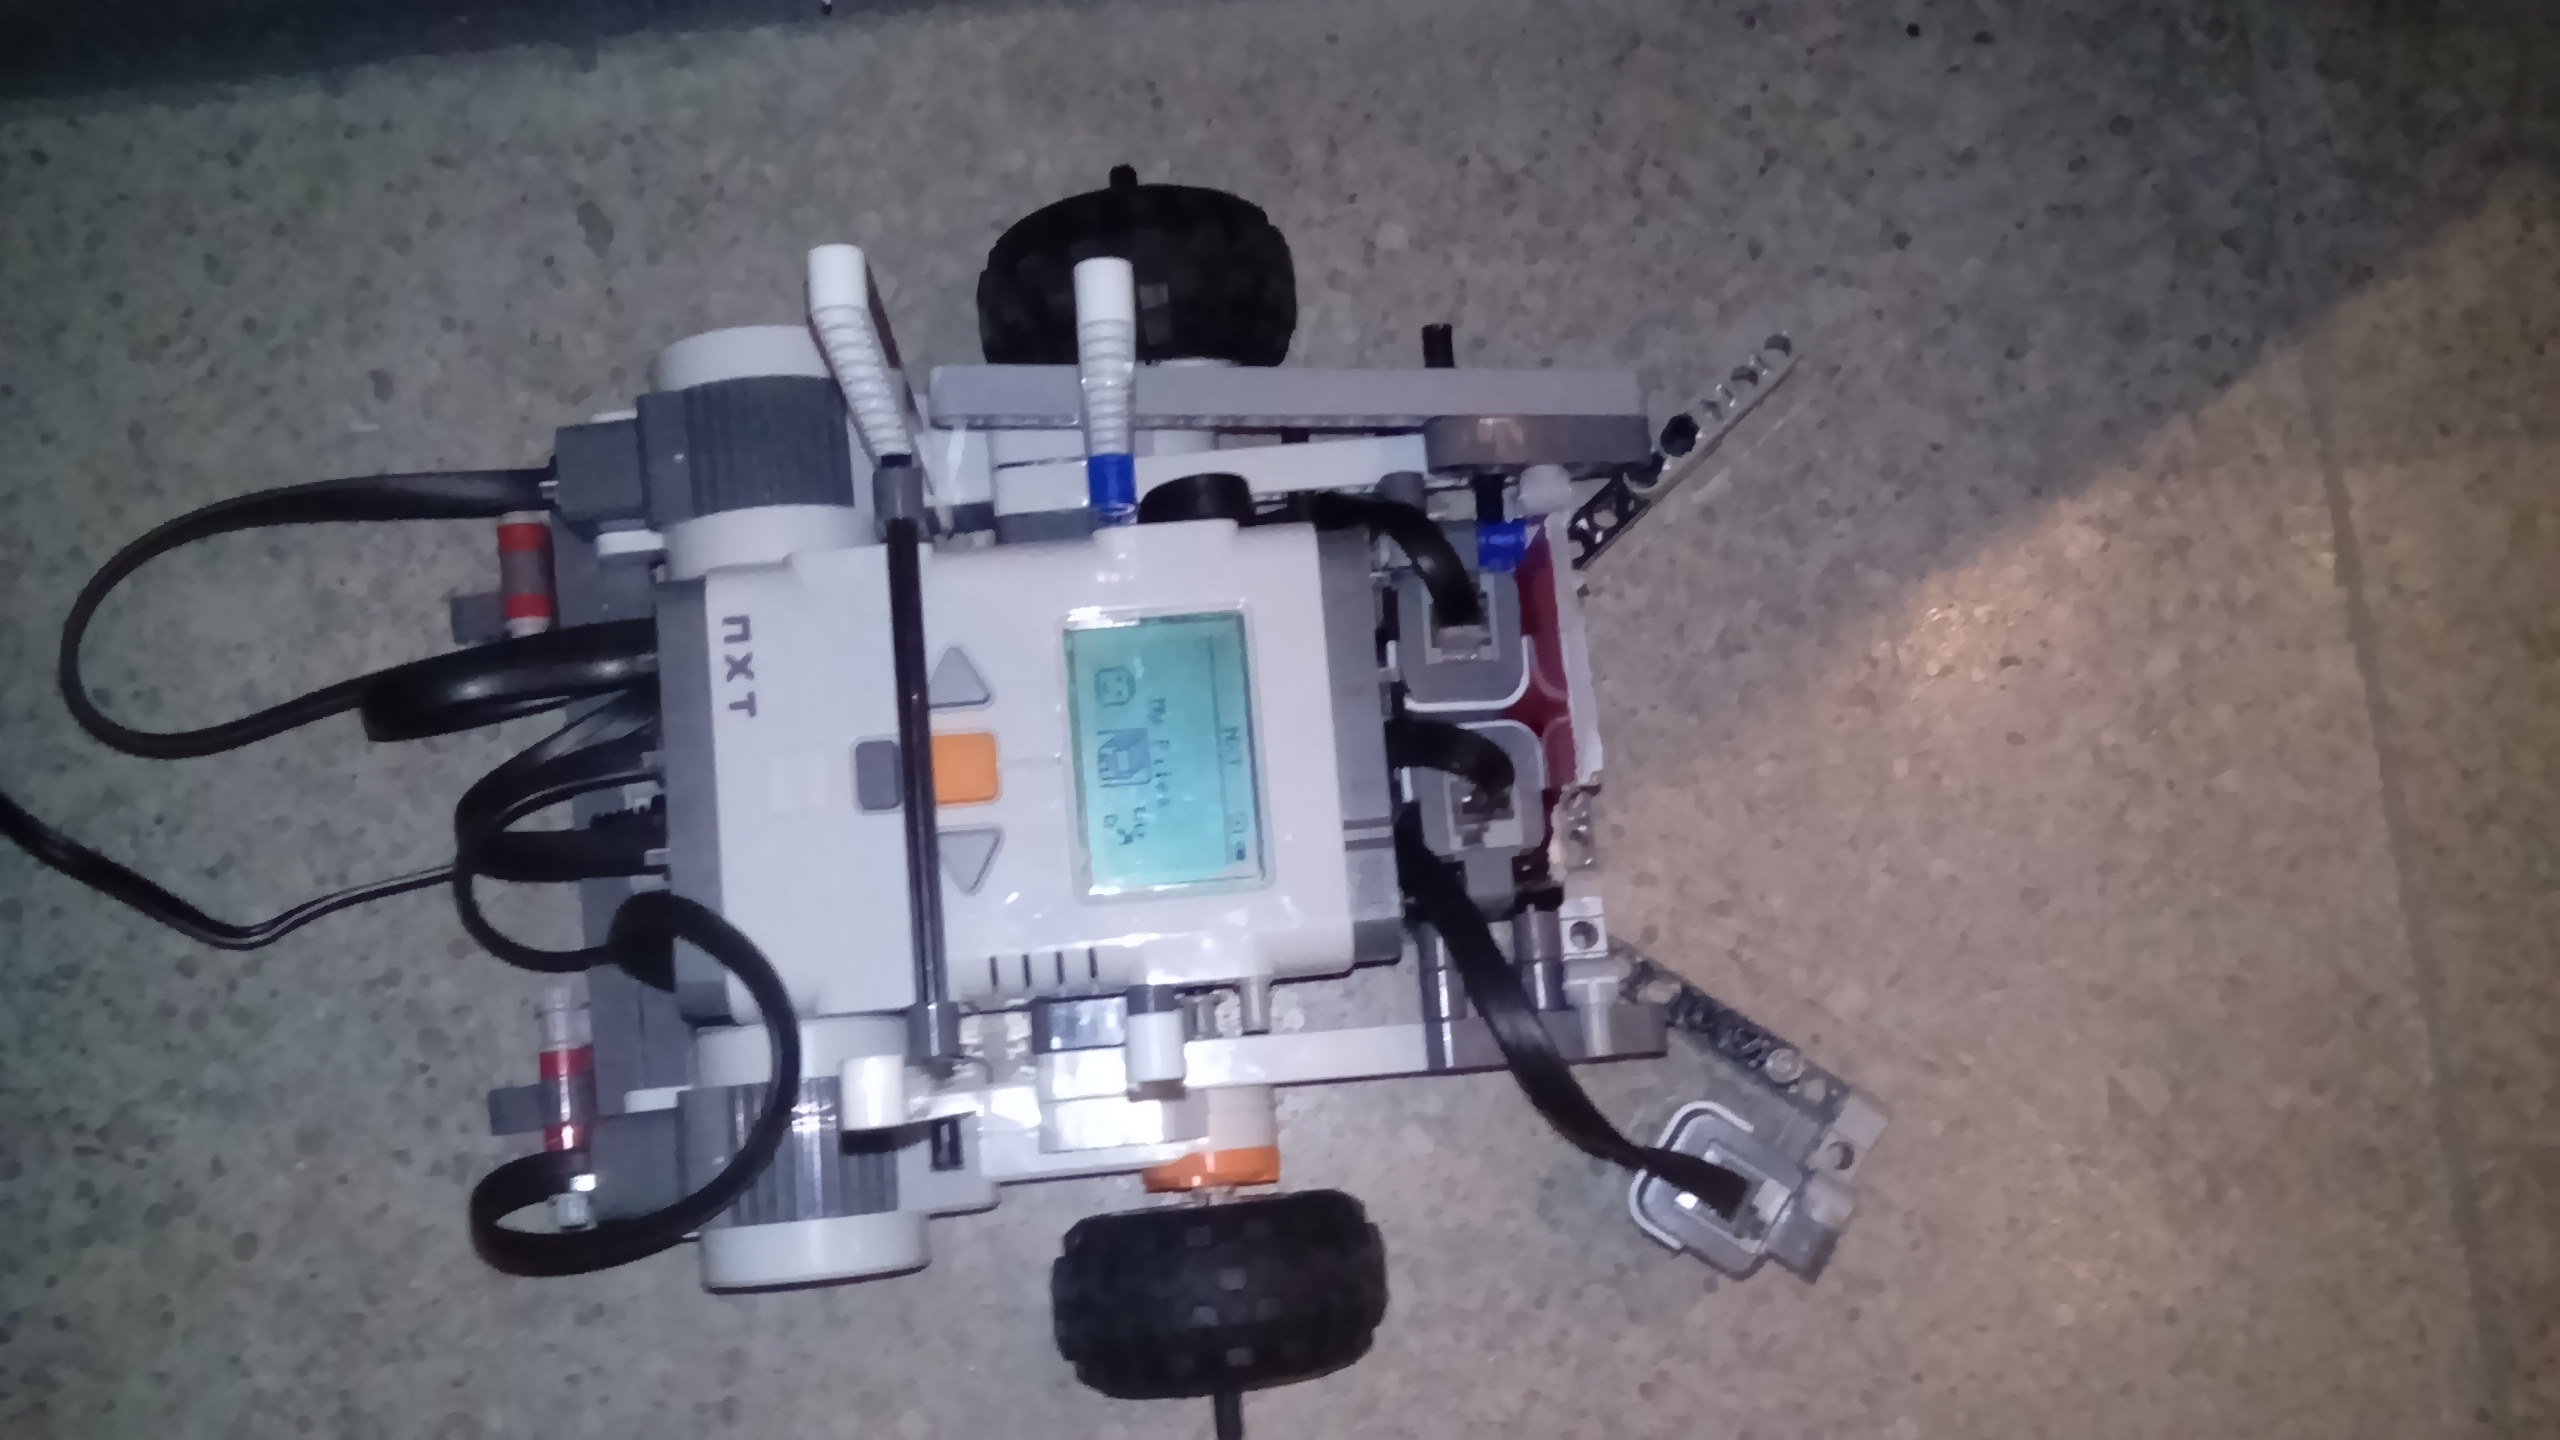
\includegraphics[scale = 0.1]{img/robot.jpg}
 \caption{Final design of the robot}
 \label{fig:final_robot}
\end{figure}


\subsection{Sensing}
In order to sense the world around it, the robot was fitted with three light sensors, the maximum number there was. Because there were only three light sensors, a decision had to be made on what to use the sensors for. All of the other types of sensors were deemed useless for this project.

The problems that needed to be addressed in the project was turning exactly 90 $^{\circ}$, and stopping with the can on the intersection.

It was quickly established that two sensors were needed for a line follow controller. The last sensor could then be used for a few things, e.g as indicator that a turn was completed or a detector of intersection. Both uses were tried and pros and cons were noted, and a decision was made on what was the best configuration.

\missingfigure{Tikz tegning af begge konfigurationer}

The first configuration, with no third sensor failed at turning enought	